\subsection{Deep Convolutional GAN (DCGAN)}
\begin{frame}{}
    \LARGE GAN Variant: \\[1.5ex] \textbf{Deep Convolutional GAN (DCGAN)}
\end{frame}

\begin{frame}[allowframebreaks]{DCGAN}
    \begin{figure}
        \centering
        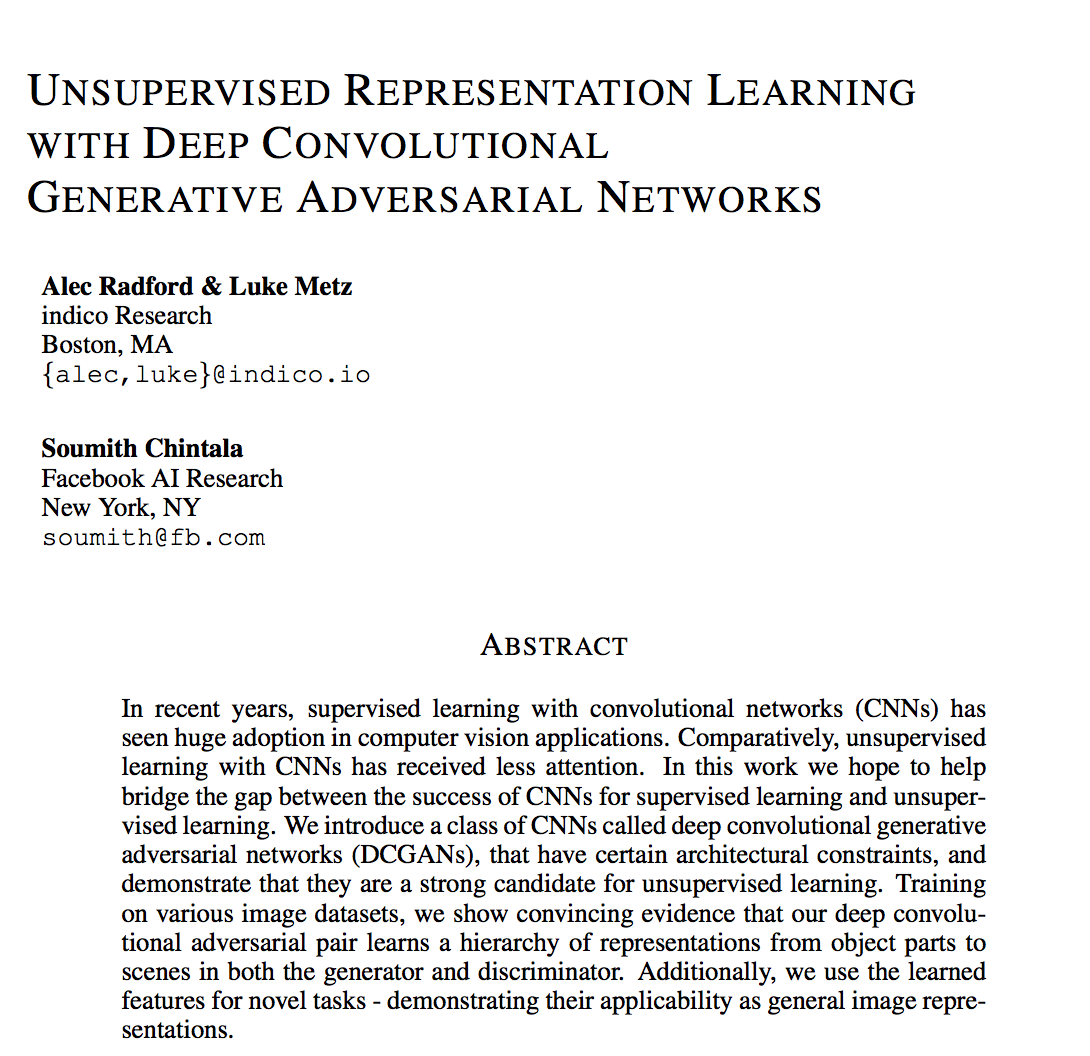
\includegraphics[height=0.9\textheight,keepaspectratio]{images/gan/dcgan-paper.png}
    \end{figure}

    \framebreak

    \begin{figure}
        \centering
        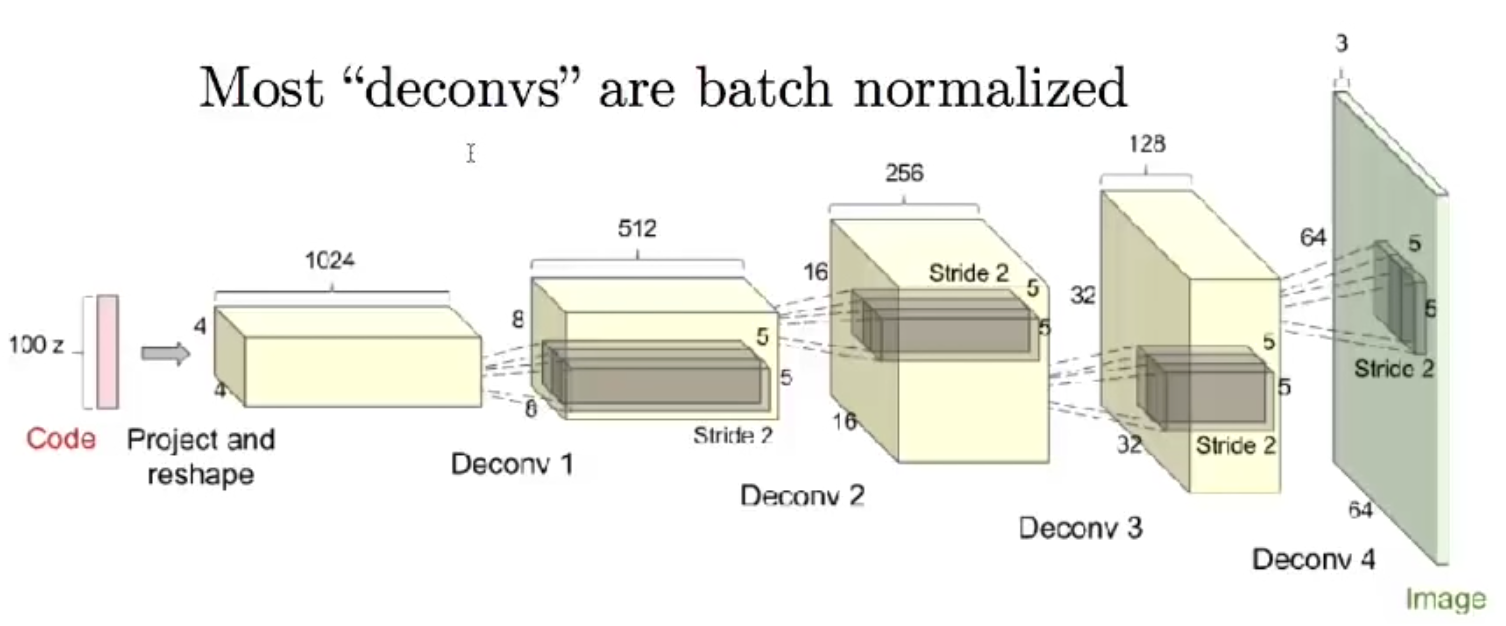
\includegraphics[width=1.05\textwidth,keepaspectratio]{images/gan/dcgan-architecture.png}
        \small [Radford et al 2016]
    \end{figure}

    \framebreak

    \textbf{Architecture Design Principles:}
    \begin{itemize}
        \item Utilizes convolutional and transposed convolutional layers instead of fully connected layers.
        \item Key architectural guidelines:
            \begin{itemize}
                \item Standard supervised CNNs are not directly usable for GANs.
                \item Remove max-pooling and mean-pooling layers.
                \item Generator upsamples using transposed convolutions.
                \item Discriminator downsamples with strided convolutions and average pooling.
                \item Non-linearity: ReLU for generator (except output), LeakyReLU (slope 0.2) for discriminator.
                \item Output non-linearity: \texttt{tanh} for generator, \texttt{sigmoid} for discriminator.
                \item Batch normalization is used to prevent mode collapse, but not applied at the output of G or input of D.
            \end{itemize}
        \item \textbf{Optimization}: Adam optimizer with learning rate $2 \times 10^{-4}$, momentum $0.5$, batch size $128$.
        \item Achieves stable training and generates high-quality images.
    \end{itemize}
\end{frame}
    
\begin{frame}[allowframebreaks]{DCGAN: Results}
    Good samples on datasets with 3M images (Faces, Bedrooms) for the first time
    \begin{figure}
        \centering
        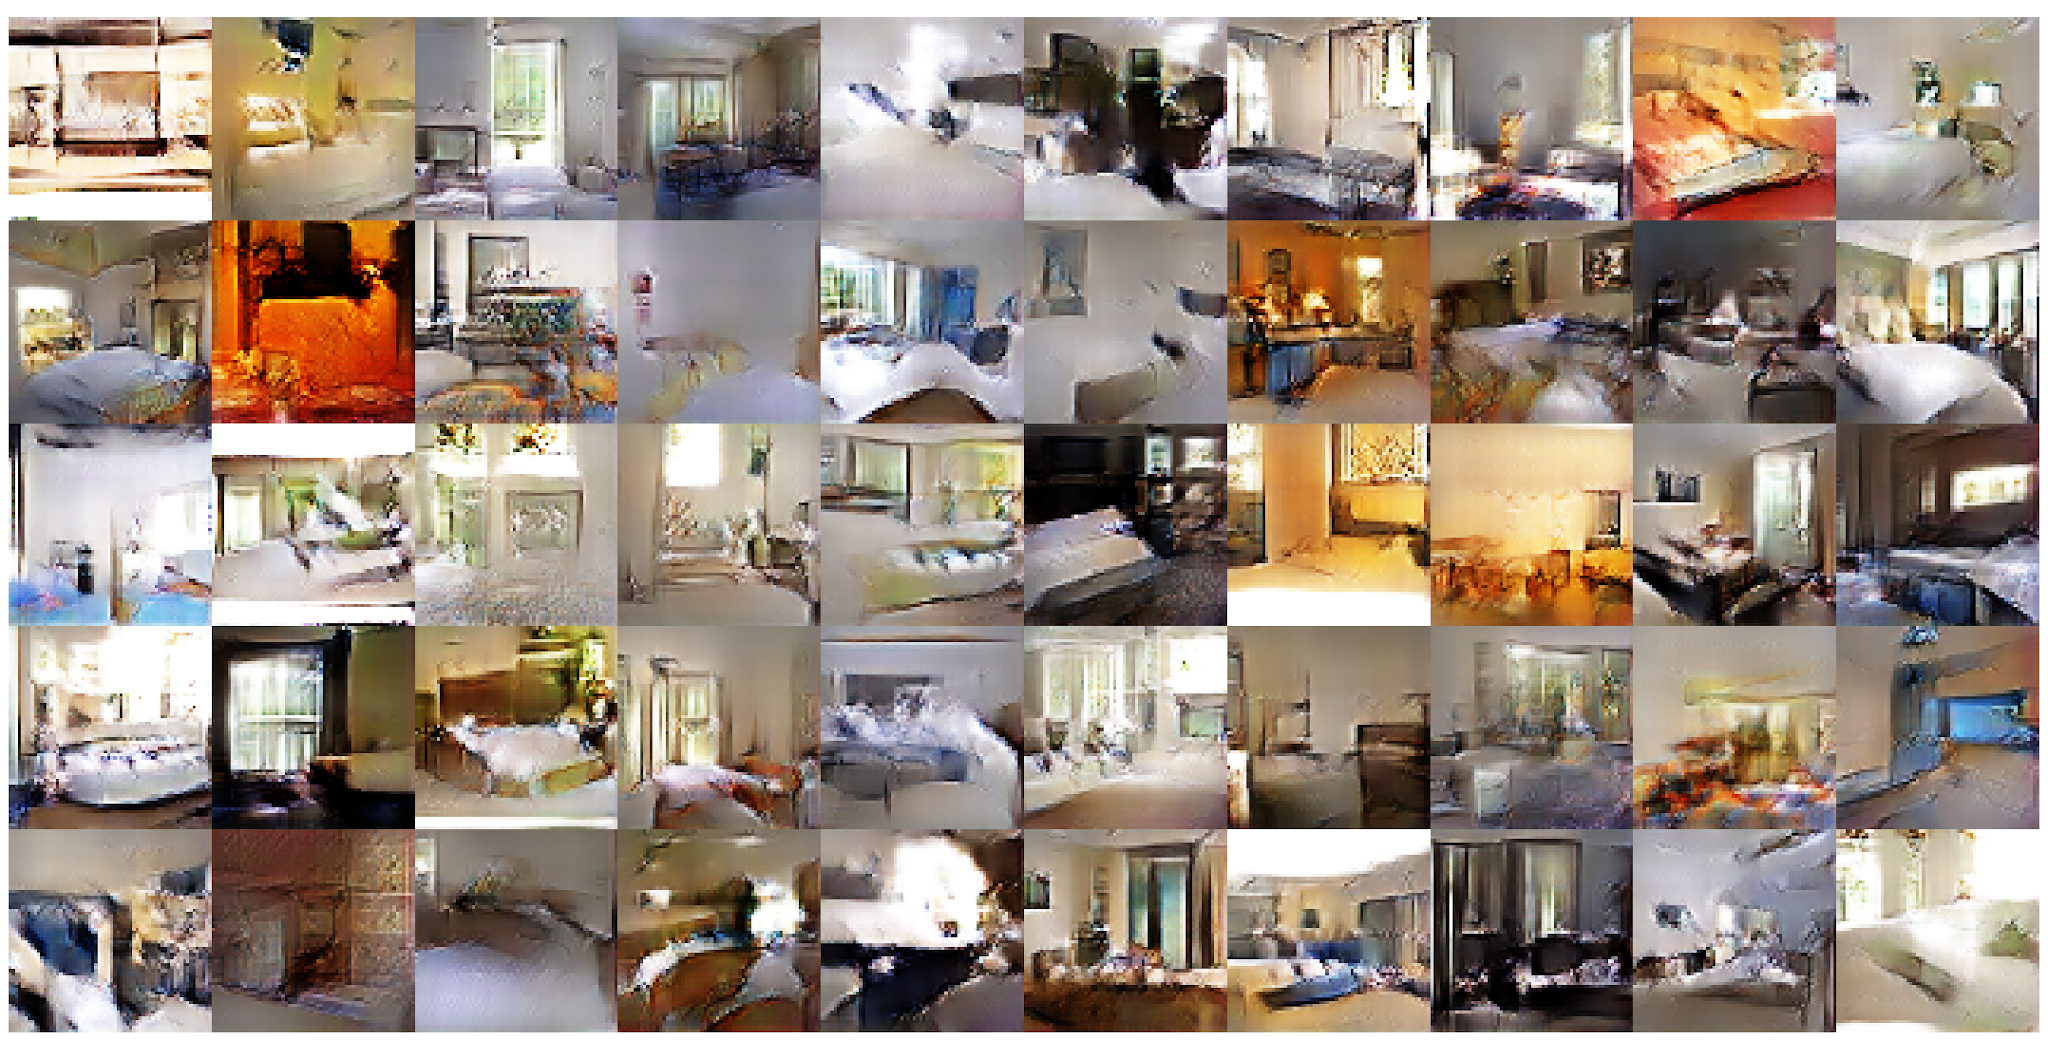
\includegraphics[width=0.9\textwidth,keepaspectratio]{images/gan/dcgan-result-1.png}
    \end{figure}
    \footnotesize{Reference: Radford, Metz, and Chintala, "Unsupervised Representation Learning with Deep Convolutional Generative Adversarial Networks", ICLR 2016}

    \framebreak

    \begin{figure}
        \centering
        \includegraphics[height=0.8\textheight,keepaspectratio]{images/gan/dcgan-result-2.png}
        \caption*{[Radford et al 2016]} 
    \end{figure}

    \framebreak

    Smooth interpolations in high dimensions
    \begin{figure}
        \centering
        \includegraphics[height=0.8\textheight,keepaspectratio]{images/gan/dcgan-result-3.png}
        \caption*{[Radford et al 2016]}
    \end{figure}

    \framebreak

    Imagenet samples (32x32)
    \begin{figure}
        \centering
        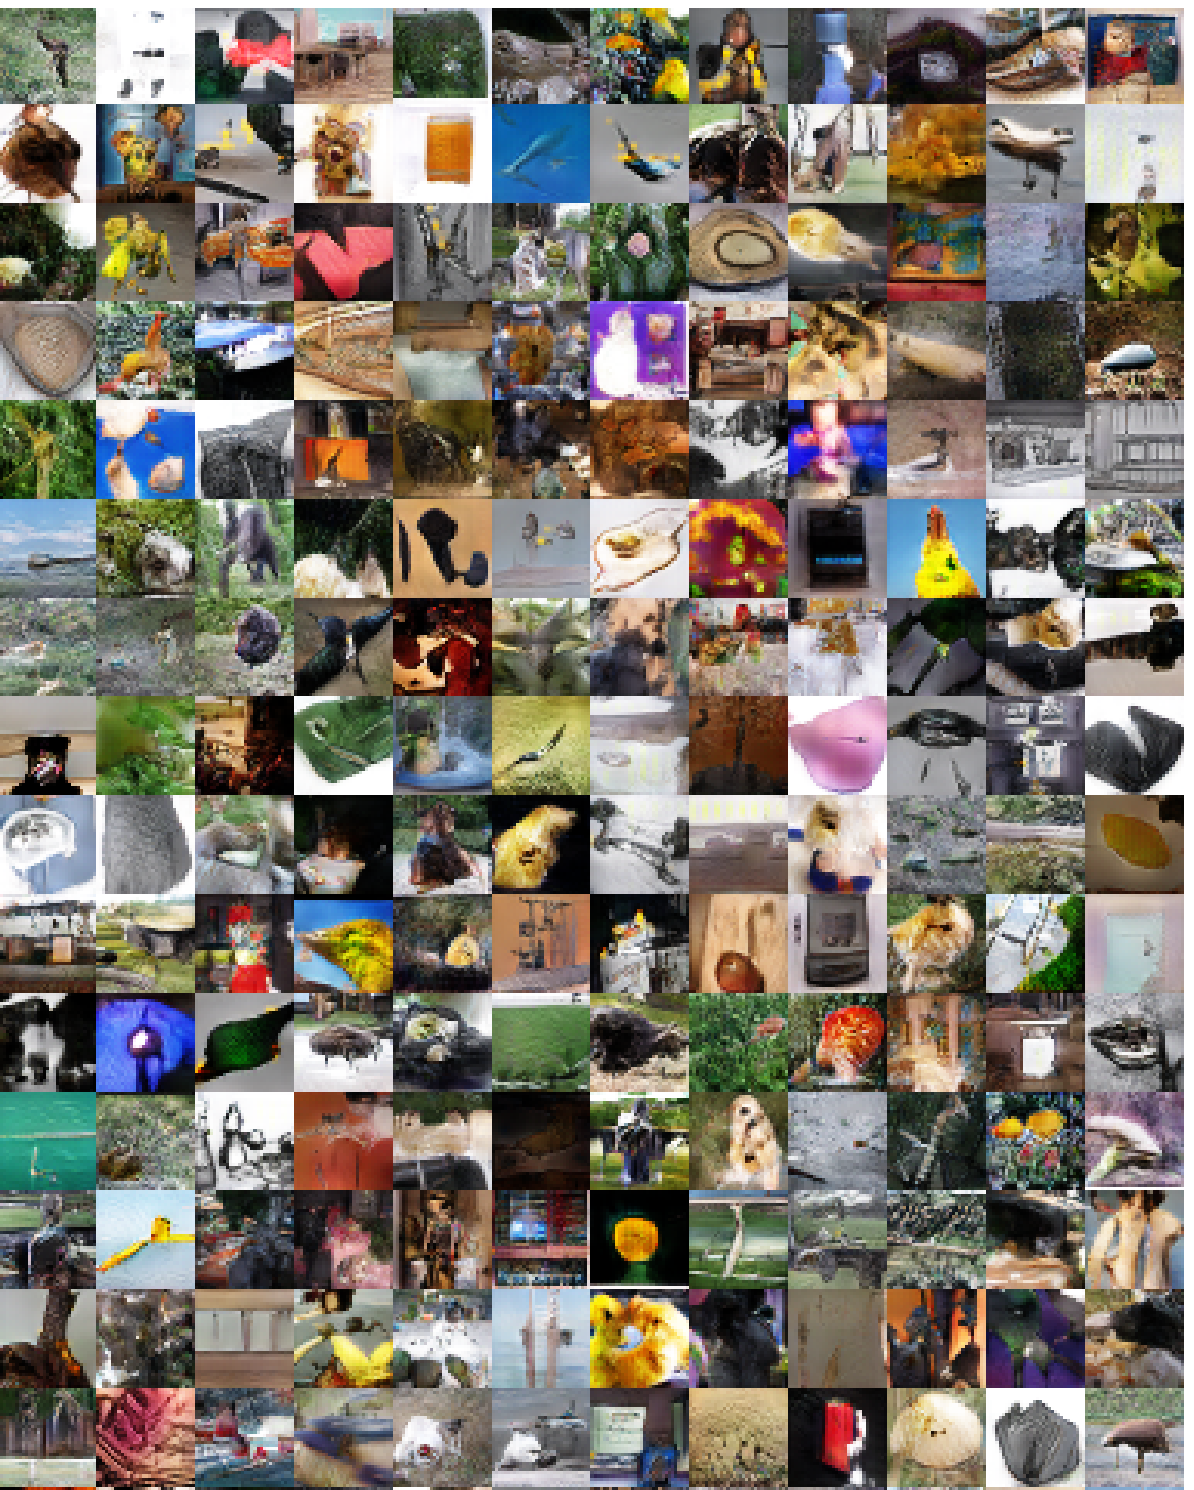
\includegraphics[height=0.8\textheight,keepaspectratio]{images/gan/dcgan-result-4.png}
        \caption*{[Radford et al 2016]}
    \end{figure}

    \framebreak

    Vector Arithmetic
    \begin{figure}
        \centering
        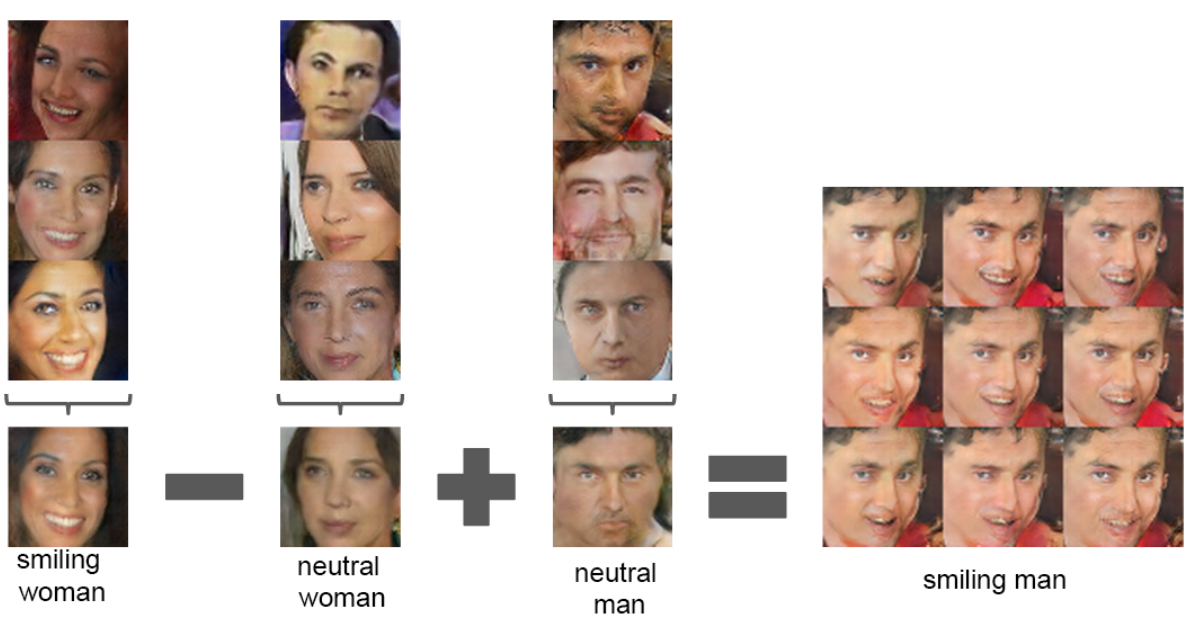
\includegraphics[height=0.75\textheight,keepaspectratio]{images/gan/dcgan-result-5.png}
        \caption*{[Radford et al 2016]}
    \end{figure}

    \framebreak

    \begin{figure}
        \centering
        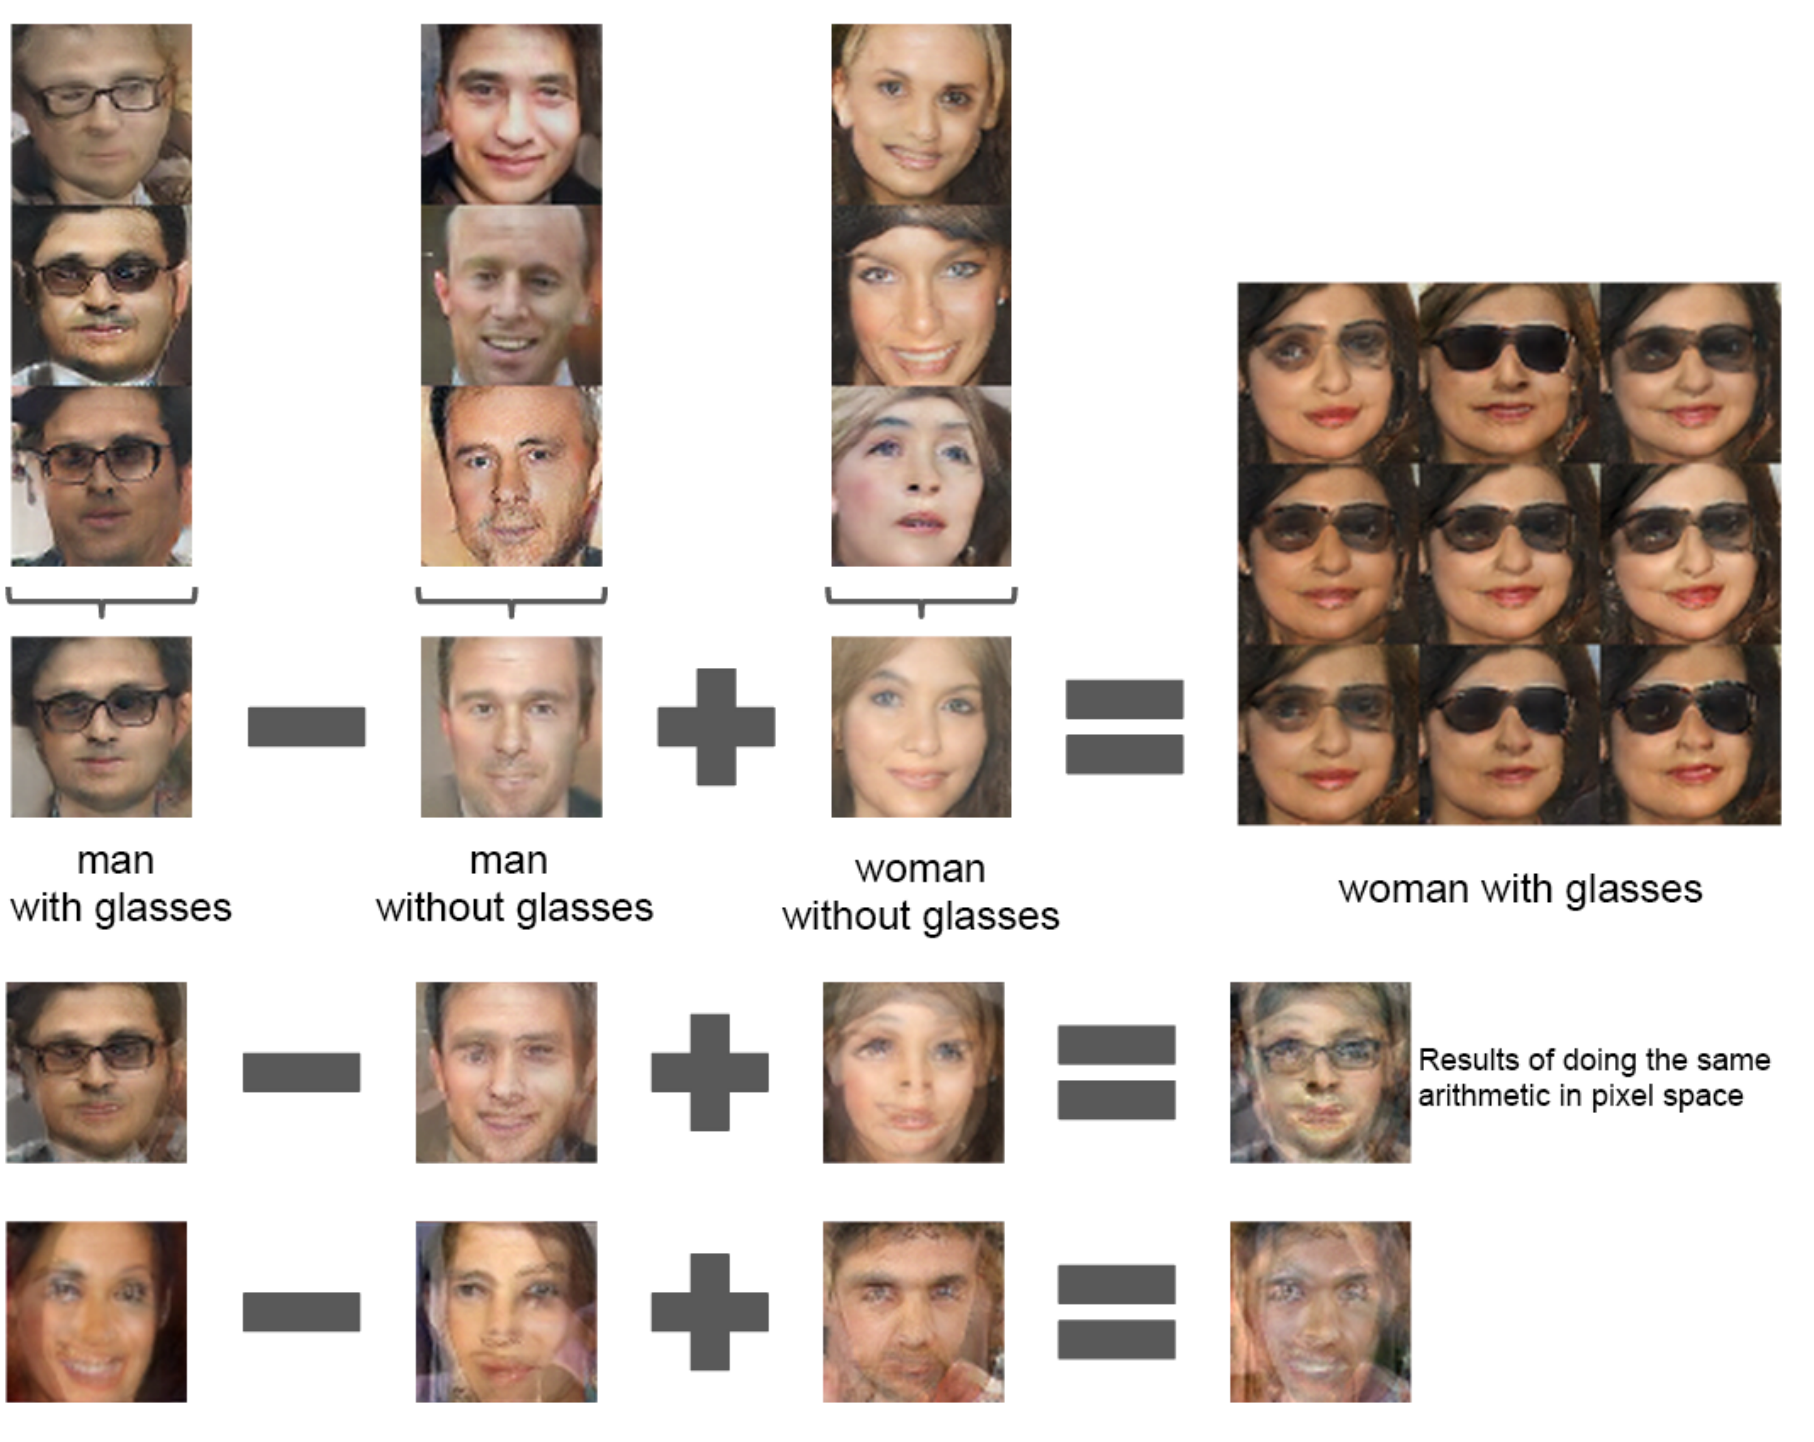
\includegraphics[height=0.8\textheight,keepaspectratio]{images/gan/dcgan-result-6.png}
        \caption*{[Radford et al 2016]}
    \end{figure}

    \framebreak

    \begin{figure}
        \centering
        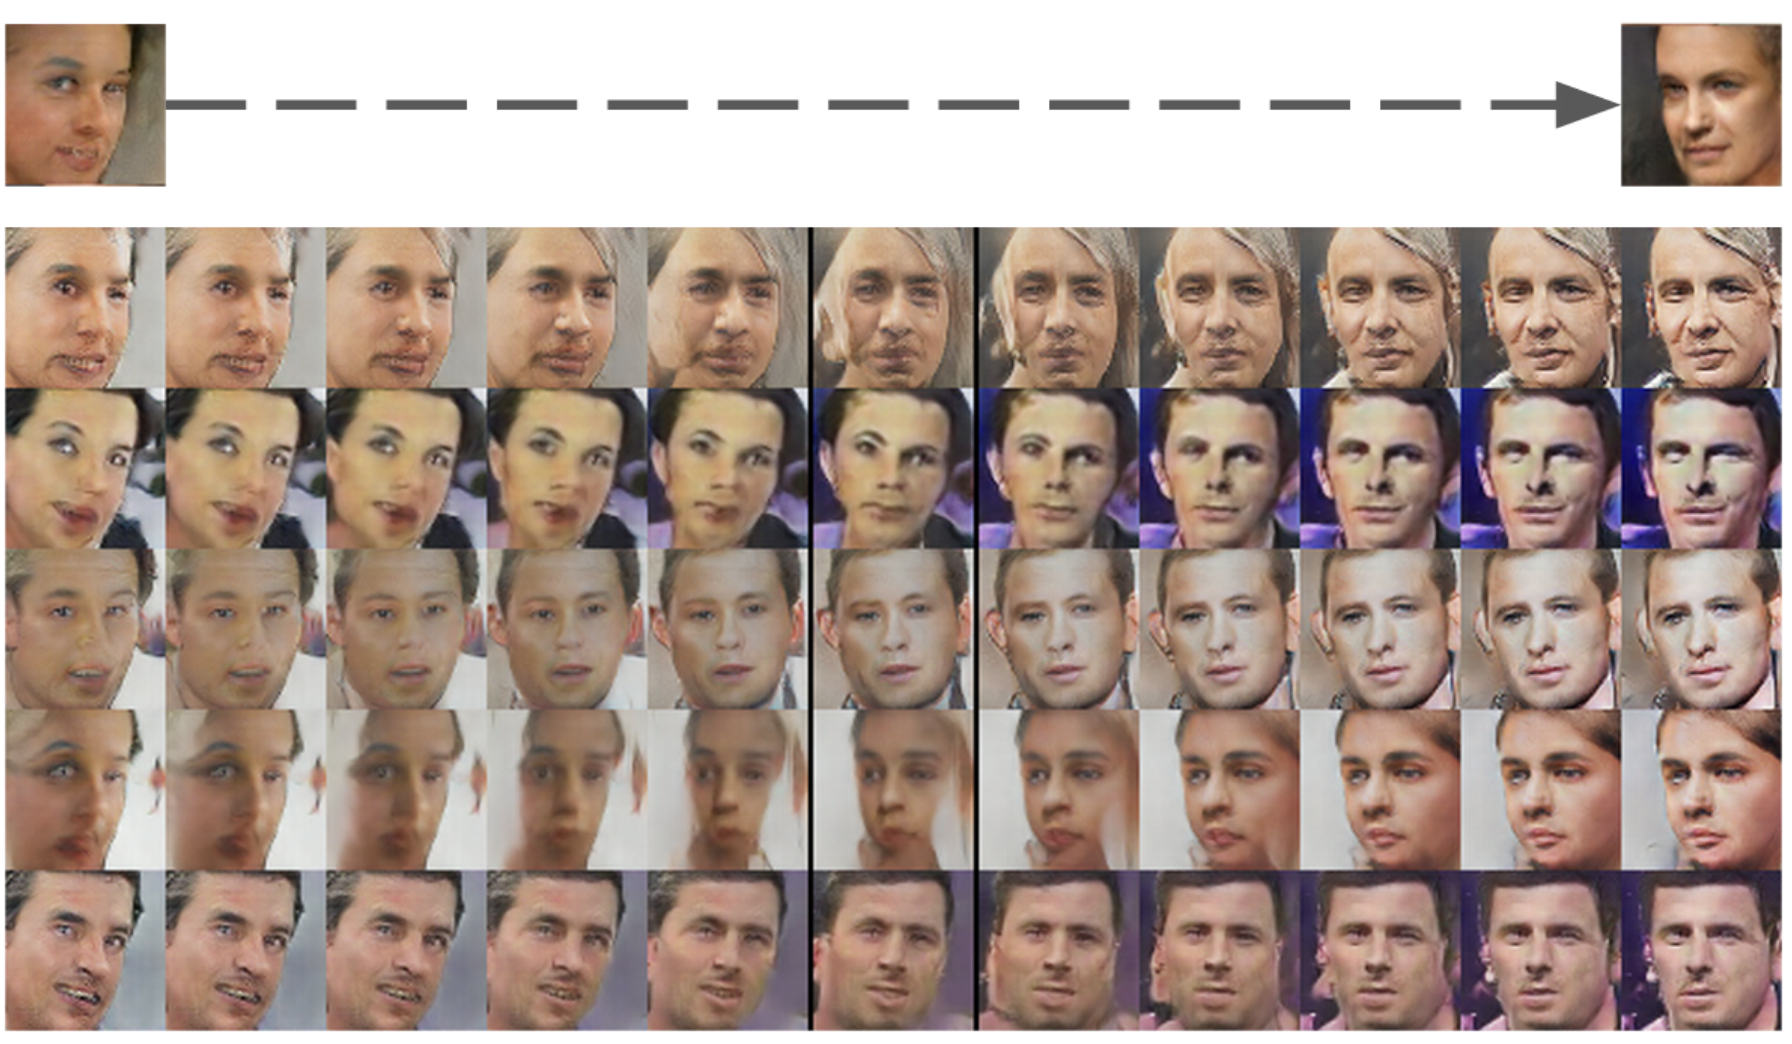
\includegraphics[height=0.8\textheight,keepaspectratio]{images/gan/dcgan-result-7.png}
        \caption*{[Radford et al 2016]}
    \end{figure}

    \framebreak

    Representation Learning 
    \begin{figure}
        \centering
        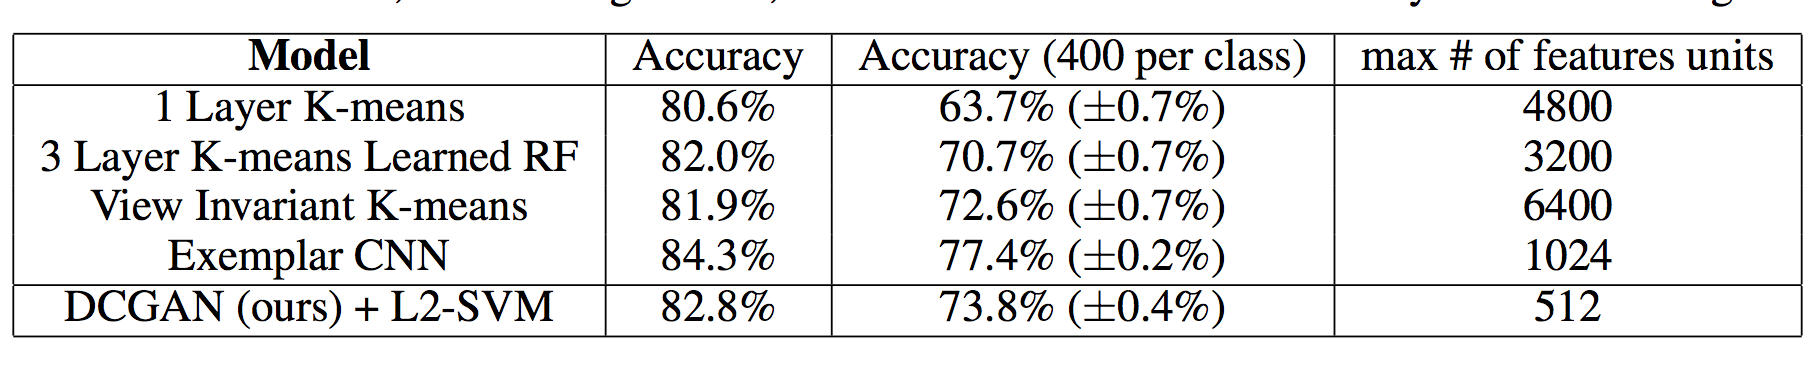
\includegraphics[width=1.05\textwidth,keepaspectratio]{images/gan/dcgan-result-table.png}
        \caption*{[Radford et al 2016]}
    \end{figure}
\end{frame}